\documentclass[11pt]{article}

\usepackage[top=16mm, bottom=16mm, left=18mm, right=18mm]{geometry}

%%%%%%%%%%%%%%%%%%%%%%%%%%%%%%%%%%
%%%%%%%		PACKAGES
%%%%%%%%%%%%%%%%%%%%%%%%%%%%%%%%%%
\usepackage{setspace} % controlling line spacing
\setlength{\parindent}{0pt} % paragraphs are not indented
\usepackage{amssymb}
\usepackage{graphicx}
\usepackage{enumitem}
\usepackage{amsfonts}
\usepackage{amssymb}
\usepackage{ifthen}
\usepackage{multicol}

\usepackage{tikz}
\usetikzlibrary{shapes, backgrounds}

\usepackage[english]{babel}

\usepackage{multicol}

\setlength{\parindent}{0cm}
%\setlength{\parskip}{1em}

\newcommand{\DS}[1]{${\displaystyle #1}$}
\newcommand{\vv}{\vspace{.5cm}}
\newcommand{\n}{\newpage}

\newcommand{\R}{\mathbb{R}}
\newcommand{\Q}{\mathbb{Q}}
\newcommand{\Z}{\mathbb{Z}}
\newcommand{\N}{\mathbb{N}}
\newcommand{\floor}[1]{\lfloor #1 \rfloor}

\definecolor{gold}{rgb}{212,175,55}
\definecolor{mygreen}{RGB}{66,165,81}
\newcommand{\azul}[1]{{\color{blue} #1}}
\newcommand{\rojo}[1]{{\color{red} #1}}
\newcommand{\verde}[1]{{\color{mygreen} #1}}

\newcommand{\set}[2]{ \left\{ #1 \; : \; #2 \right\} }
\newcommand{\e}{\varepsilon}

%\newcommand{\DS}[1]{${\displaystyle #1}$}

\definecolor{137cp1}{RGB}{13, 33, 161}
\definecolor{137cp2}{RGB}{51, 161, 253}
\definecolor{137cp3}{RGB}{255, 67, 101}%{255, 84, 0}
\definecolor{137cp4}{RGB}{232, 144, 5}%{255, 190, 11}%{83, 221, 108}%{38, 196, 133}

\usepackage{hyperref}
\hypersetup{colorlinks}
\hypersetup{urlcolor=137cp3, linkcolor=137cp1}

\usepackage{sectsty}
\sectionfont{\centering \LARGE\color{137cp3}} % sets colour of chapters
\subsectionfont{\Large \color{137cp2}}
\subsubsectionfont{\large \color{137cp4}}
\paragraphfont{\color{137cp1}}

\usepackage{tikzsymbols}
\usepackage[final]{pdfpages} %insert .pdf file

\setcounter{secnumdepth}{0}
\setcounter{tocdepth}{2}

%% BOXES
\usepackage[most]{tcolorbox}

\usepackage{amsthm, thmtools}
\usepackage{mdframed}

% kill warnings for overfull hboxes
\newcommand{\ignoreoverfullhboxes}{\setlength{\hfuzz}{\maxdimen}}
\AtBeginEnvironment{mdframed}{\ignoreoverfullhboxes}

%==========================================
%: theorem styles
%==========================================

\declaretheoremstyle[
spaceabove=-6mm,
spacebelow=-2cm,
headfont=
\color{137cp1}
\bfseries,
notefont=\bfseries\mathversion{bold},
notebraces={(}{)},
postheadspace=2mm,
headpunct={.}
]{myexample}

\declaretheoremstyle[
spaceabove=-6mm,
spacebelow=-2cm,
headfont=
\color{137cp1}
\normalfont,
bodyfont=\normalfont,
postheadspace=2mm,
headpunct={.}
]{myparts}

%==========================================
%: theorem environments
%==========================================
% ??? create theorem synopsis - list of only important theorems/prop/lem - environments with option to add to this list

\definecolor{Lavender}{rgb}{0.95,0.90,1.00}
\definecolor{darkviolet}{rgb}{0.35,0.00,0.70}

\newcommand{\mypartscolour}{Lavender!30}
\newcommand{\mylemmacolour}{darkviolet!15}
\newcommand{\mydefinitioncolour}{red!50}
\newcommand{\myremarkcolour}{yellow!25}

%: 	EXAMPLE

\declaretheorem
[style=myexample,
name=Example,
refname={Example},
Refname={Example},
]
{thmx}

\DeclareDocumentEnvironment{example}{O{ } g} % optional arguments: title, label
{\begin{mdframed} [backgroundcolor=\mypartscolour, skipabove=0.5\baselineskip, innertopmargin=0.5\baselineskip, skipbelow=0.5\baselineskip, innerbottommargin=0.1\baselineskip, roundcorner=12pt leftmargin=0.25cm, rightmargin=-0.25cm, innerleftmargin=0.3cm, innerrightmargin=0.25cm, linewidth=4pt, linecolor=137cp1, hidealllines=true, leftline=true, nobreak=false, roundcorner=50pt ] \begin{thmx}[#1] \IfNoValueTF{#2}{}{\label{#2}\hypertarget{#2}{}}}
{\end{thmx} \end{mdframed}}

%: 	BACKGROUND
\declaretheorem
[style=myparts,
name=Background,
numbered=no]
{propx}

\DeclareDocumentEnvironment{background}{O{ } g} % optional arguments: title, label
{\begin{mdframed} [backgroundcolor=\mypartscolour, skipabove=0.5\baselineskip, innertopmargin=0\baselineskip, skipbelow=0\baselineskip, innerbottommargin=0.5\baselineskip, leftmargin=-0.25cm, rightmargin=-0.25cm, innerleftmargin=0.25cm, innerrightmargin=0.25cm, linewidth=3pt, linecolor=137cp3, hidealllines=true, leftline=true, nobreak=false] \begin{propx}[#1]%
\IfNoValueTF{#2}{}{\label{#2}\hypertarget{#2}{}}}
{\end{propx} \end{mdframed}}

%: 	QUESTION
\declaretheorem
[style=myparts,
name=Question,
numbered=no]
{corx}

\DeclareDocumentEnvironment{question}{O{ } g} % optional arguments: title, label
{\begin{mdframed} [backgroundcolor=\mypartscolour, skipabove=0\baselineskip, innertopmargin=0.5\baselineskip, skipbelow=0\baselineskip, innerbottommargin=0.5\baselineskip, leftmargin=-0.25cm, rightmargin=-0.25cm, innerleftmargin=0.25cm, innerrightmargin=0.25cm, linewidth=3pt, linecolor=137cp2, hidealllines=true, leftline=true, nobreak=false] \begin{corx}[#1]%
\IfNoValueTF{#2}{}{\label{#2}\hypertarget{#2}{}}}
{\end{corx} \end{mdframed}}

%: 	COMMENTS
\declaretheorem
[style=myparts,
name=Comments,
numbered=no]
{comm}

\DeclareDocumentEnvironment{comments}{O{ } g} % optional arguments: title, label
{\begin{mdframed} [backgroundcolor=\mypartscolour, skipabove=0\baselineskip, innertopmargin=0.5\baselineskip, skipbelow=1\baselineskip, innerbottommargin=0.5\baselineskip, leftmargin=-0.25cm, rightmargin=-0.25cm, innerleftmargin=0.25cm, innerrightmargin=0.25cm, linewidth=3pt, linecolor=137cp4, hidealllines=true, leftline=true, nobreak=false] \begin{comm}[#1]%
\IfNoValueTF{#2}{}{\label{#2}\hypertarget{#2}{}}}
{\end{comm} \end{mdframed}}

\renewcommand{\labelitemi}{$\textcolor{137cp1}{\bullet}$}

\usepackage{fancyhdr}
\renewcommand{\headrulewidth}{.4mm} % header line width
\pagestyle{fancy}
\fancyhf{}
\fancyhfoffset[L]{1cm} % left extra length
\fancyhfoffset[R]{1cm} % right extra length
\lhead{\textcolor{137cp1}{MAT137Y Instructor Guide}}
\rhead{\scshape\nouppercase{\textcolor{137cp1}{\leftmark}}}
\rfoot{}
\cfoot{\thepage}

%%%%%%%%%%%%%%%%%%%%%%%%%%%%%%%%%%%%%%%%%

\begin{document}
	\thispagestyle{empty}
	\phantom{.}
	\vspace{3cm}
	\begin{center}
		{ \fontsize{30}{28}\selectfont \textcolor{137cp3}{ {\bf MAT137Y }}\\[0.5\baselineskip]

		{\textcolor{137cp3}{ {\fontsize{20}{20} \scshape Instructor Guide:\\[0.5\baselineskip] Inverted Class}}} }\\[2\baselineskip]

		{\Large \bf \textcolor{137cp1}{Alfonso Gracia-Saz and Beatriz Navarro-Lameda} }
	\end{center}

	\vspace{0.5cm}

	\begin{center}
		\begin{minipage}{0.7\textwidth}
			This guide is for new MAT137Y instructors who perhaps are teaching an inverted
			class for the first time. It is normal to be confused, intimidated, or
			even skeptical at first. We hope this guide will provide you with the necessary
			tools for you to feel more confident, and will make the picture of an
			inverted class much more concrete.
		\end{minipage}

		\vspace{1cm}

		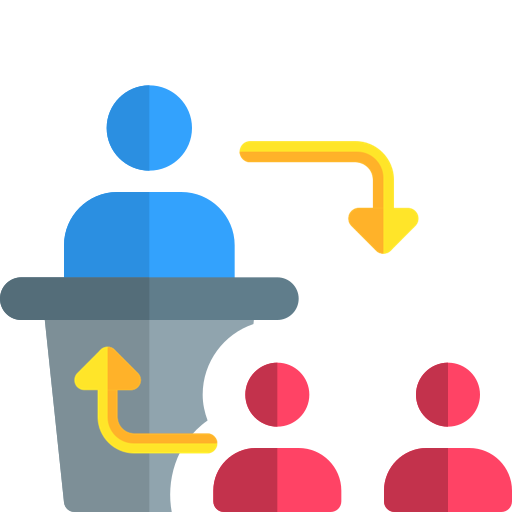
\includegraphics[width=0.5\textwidth]{flippedclass}
	\end{center}

	\newpage

	This document is divided into three main sections:

	\paragraph{\hyperref[sec:general]{Inverted Class: General Aspects.}}
	This section focuses on the general aspects of an inverted class. If you are not
	familiar with the term inverted class or you are skeptical about the effectiveness
	of an inverted class, we strongly encourage you to read this section first. You
	will find answers to questions like:

	\begin{itemize}
		\item What is an inverted course?
			\vspace{-1mm}

		\item How is an inverted class different from a traditional lecture?
			\vspace{-1mm}

		\item What exactly happens in an inverted class?
			\vspace{-1mm}

		\item Why do it? Why not lecture?
			\vspace{-1mm}

		\item Does it work?
	\end{itemize}

	\paragraph{\hyperref[sec:structure]{Inverted Class: MAT137 Implementation.}}
	The second section focuses on the implementation of an inverted course model specifically
	in the context of MAT137. We explain the structure of MAT137Y, what happens in
	class, and we offer some advice.

	\paragraph{\hyperref[sec:activities]{Commentated Examples of In-class
	Activities.}}
	This section, covering more than half of this guide, contains lots of concrete
	example of class activities with a commentary providing some background,
	explaining how to use the sample activities, and what to expect from students.

	\tableofcontents

	\newpage

	\renewcommand{\baselinestretch}{1.3} %increase line spacing

	%==================
	%==================

	\section[1. Inverted Class: General Aspects]{Inverted Class: General Aspects}
	\label{sec:general}

	%==================
	%==================

	\subsection{A learning model}
	\label{sec:model}

	Here is a rough (made up) model of how a student learns a math concept. I
	claim it goes in three steps:
	\paragraph{First Contact.}
	The student learns the basics of the materials for the first time. This part is
	passive: the student either reads this or watches somebody explain it. These are
	the steps necessary before the student can start actively ``doing" math by
	themself with the new concept. They could be receiving an explanation or motivation
	on why the concept is important, learning the basic definitions, reading statements
	of theorems for the first time, seeing examples worked out for the first time,
	memorizing an algorithm, or something else.
	\paragraph{First Practice.}
	The student engages with the material for the first time. This part is active:
	the student is doing the math themself, perhaps collaborating with other students
	or assisted by us. Through this process, the student gains intuition about the
	concepts. They could be performing computations, thinking about how concepts relate
	or what is true or false, coming up with conjectures, trying to prove results,
	looking for errors in proofs, constructing examples or counterexamples, or
	many other things.
	\paragraph{Deep Practice.}
	The student tackles harder problems and thinks deeply about them, probably struggling
	with them through a longer period of time. This part is very active. It helps solidify
	their understanding and sharpen their skills.

	\
 Any mathematician will recognize ``Deep Practice" as the part when we
	actually learn a concept for real, the only way to achieve understanding. We
	should also recognize that of the three steps, ``First Contact" is by far the
	easiest, and the one for which students need us the least.

	%==================
	%==================

	\subsection{Lectures, active learning, and an inverted class}

	\paragraph{Lecture-based class $\equiv$ First Contact.}
	I define a \emph{traditional class} or a \emph{lecture-based class} as a class
	where most of the time is spent with the instructor presenting something on
	the board (or on slides) while students listen and/or take notes. This could include,
	for example, the instructor proving theorems, performing calculations, or giving
	motivation.

	{\parskip=0.5\baselineskip In a lecture-based course all the class time (or almost all the class time) is spent on the first step: First Contact. Students may or may not be understanding on real time, and they may or may not be taking notes. We hope that students will do the other two steps later at home by themselves. }

	\paragraph{Active-learning class $\equiv$ First Practice.}
	I define an \emph{active-learning class} as a class where most of the class
	time is spent with students doing math themselves, rather than watching the instructor
	do it. There are many forms of active learning. In an \emph{\textcolor{137cp1}{inverted
	class}} or \emph{\textcolor{137cp1}{flipped class}} students spend the majority
	of their class time working on First Practice, through carefully prepared
	activities, alone or collaborating with their peers, with our guidance. In order
	for this to work, students need to take care of First Contact before coming to
	class, as ``pre-homework". They will normally watch videos or read material ahead
	of time so that when class starts we can assume they have the basics and they can
	start practicing right away.

	%==================
	%==================

	\newpage

	\subsection{Why we don't lecture anymore in MAT137Y}
	\label{sec:nolec}

	\paragraph{No longer necessary.}
	Lecturing is a very old form of teaching. It has its origins at a time when
	information was not readily available, not only before modern technology and the
	internet, but back when duplicating, making copies, or even finding books was
	difficult. The purpose of a lecture was simply to provide students with a set of
	notes they could learn from. The instructor presented the material and the
	students copied it; they would use it as a reference to study later. Lectures
	are no longer necessary for this specific purpose. Moreover, they only serve
	as First Contact, the first step in the learning model above. It seems a waste
	to spend the precious little time we have with students with the easiest of
	the three steps, the one students need us the least for, and then leaving them
	alone for the rest of the process.

	\paragraph{Not a good way to absorb material.}
	Secondly, as a way of absorbing the material, physical real-time lectures do not
	work, particularly in the setting of a large calculus class with 200 students,
	each with a different pace. Think about the research seminars or conferences
	you have attended. Have you ever been unable to follow one such seminar because
	the presenter was going too fast, because they proceeded to write a complex
	proof with a concept they had just defined without giving you time to absorb
	the definition and develop intuition about it? That is the experience of the average
	undergraduate student, who is not a math major, in a math class. Chances are
	you are going too fast for them to follow on real time, to think about the material
	at the same time as you speak it, to convince themselves that what you are
	saying is true. By and large, for the purpose of First Contact, students much rather
	prefer watching videos with the same material which they can pause, rewind, and
	come back to as needed.

	\paragraph{Lack of student feedback.}
	Thirdly, it is very easy to convince yourself that students have learned something
	that they have not, or that their understanding is much better than it
	actually is. We pretty much do it every single time we lecture, particularly
	if we are good lecturers. Think back to your lecturing experience: have you
	ever delivered a fantastic lecture on a specific concept, well crafted and structured,
	with crystal-clear explanations, that perfectly explains the important points,
	only to find out on the exam that half the students did not get the most basic
	point and made the error you warned them of? If you have been lecturing for a while,
	I am certain this will be familiar. The evidence that students did not learn something
	just because we lectured well on it was there all the time, but we continued
	ignoring it and repeating the same lecture as though it worked.

	{\parskip=0.5\baselineskip By contrast, when students do not understand a concept in an inverted classroom, the evidence is in your face and you cannot ignore it. By its own structure, you are receiving constant feedback from the students on every activity, so you know what they do not get and which errors they make. This can be overwhelming at first; sometimes ignorance is bliss and we may wish we could go back to pretending they had gotten it and moving on, but it is important to remember that this feedback is a feature, not a bug. You want to know if your explanations are not working, don't you?\\ }

	\begin{example}
		\label{even} {\parskip=0.5\baselineskip When I used to lecture in MAT137Y, after introducing the quantifiers $\forall$ and $\exists$, I would give some simple examples of how to use them in definitions. This would include
		%
		\begin{center}``Definition: Let $a \in \mathbb{Z}$. We say that $a$ is even when $\exists b \in \mathbb{Z}$ such that $a=2b$".\end{center}
		%
		I always assumed this was a very basic, simple example that nobody would have trouble with, and I immediately moved to more interesting statements, such as those with two quantifiers.

		\newpage When I inverted the class for the first time, I instead asked students to complete the definition:
		%
		\begin{center}``Definition: Let $a \in \mathbb{Z}$. We say that $a$ is even when ..."\end{center}
		%
		To my surprise the class was split between two options: \begin{itemize}\item ``... $\exists b \in \mathbb{Z}$ such that $a=2b$"

		\item ``... $\forall b \in \mathbb{Z}$, $a=2b$"\end{itemize} I repeated the question every year ever since, so have other instructors, and we always have the same result. Yet none of us would have ever thought of it! Why do students make this error? They are thinking that it is true that ``$\forall b \in \mathbb{Z}$ the number $a=2b$ is even". But that is a claim or theorem, not the definition we were aiming for. They do not understand what a definition is; the notion of definition is much deeper and harder to absorb that we thought at first. Without an inverted class, we would have never found out.

		Here is how I use this exercise nowadays. I first ask students to individually complete the definition. Afterwards, I offer the two options and ask them to vote. The vote is normally split fifty-fifty. Then I tell students to discuss it with their neighbour. They are now eager to discuss and they do so, because they had mostly answered with confidence and they are suprised that half the class disagreed with them. After a minute I ask them to vote again. Sometimes they have now convinced each other and converged to the right answer, so we can move on. But sometimes they have not. In that case, I give them the hint ``Is the number $a=6$ even? Does $a=6$ satisfy the definition?" Now they discuss again, and then they re-vote. By this time they have reached the right consensus. To finish, I remind them of what a definition is. }
	\end{example}

	\paragraph{Passive.}
	Finally, there is one additional advantage of an inverted class. We are instilling
	good habits into our students. They take ownership of their math learning, as opposed
	to being passive spectators. They get used to working on math regularly, a few
	times each week. They get used to collaborating and discussing with other
	students. And they see the difference that it makes to come to class prepared.
	By contrast, in a traditional class they can convince themselves that they are
	``doing their part" as long as they come to class and take notes, even if they
	have no idea what is going on and they are just transcribing without understanding.

	\subsection{What does the research say?}
	{\parskip=0.5\baselineskip In 2016 the Conference Board of Mathematical Science (CMBS), an umbrella organization consisting of 17 professional mathematical associations in the US (including the AMS and the MAA), upon thorough analysis or studies and meta-studies, issued a statement calling {``on institutions of higher education, mathematics departments and the mathematics faculty, public policy-makers, and funding agencies to invest time and resources to ensure that effective active learning is incorporated into post-secondary mathematics classrooms"}. They define active learning as ``classroom environments in which students are provided opportunities to engage in mathematical investigation, communication, and group problem-solving, while also receiving feedback on their work from both experts and peers".

	To learn what the research says on active learning, I recommend the \href{https://www.cbmsweb.org/2016/07/active-learning-in-post-secondary-mathematics-education/}{references in their report}. }

	%==================
	%==================

	\newpage

	\section[2. Inverted Class: MAT137Y Implementation]{Inverted Class: MAT137Y Implementation}

	\subsection{The MAT137Y structure}
	\label{sec:structure}

	Students have videos to watch before class. They meet with you for class (what
	used to be lectures) for three weekly hours, and with a TA in a small tutorial
	for one weekly hour. In 2020-2021, while teaching is online, we are replacing tutorials
	with additional office hours. Students also have practice problems, problem sets
	to be submitted, and tests. They can get help in office hours, or at our
	piazza online forum. The course coordinator deals with most of the logistics of
	the course.

	\subsection{Resources for students}

	\paragraph{Course Website.}
	This is the central place where all information, resources, and links about the
	course appear. It may be on Quercus or perhaps on a separate website. The course
	website is \textbf{maintained by the course coordinator} for all students in
	all sections of the course. Don't replicate this.
	\paragraph{Course Outline.}
	This document explains all the administrative aspects of the course,
	expectations, and assessment.
	\paragraph{Videos.}
	There is a library of short \href{https://www.youtube.com/channel/UCLzpR8AiHx9h_-yt2fAxd_A/playlists}{YouTube
	videos}, created specifically for this course, that students are expected to watch
	before each class.
	\paragraph{Practice Problems.}
	There is a collection of practice problems for each unit, with short answers.
	\paragraph{No Required Textbook.}
	The videos plus the practice problems remove the need for a textbook. There is
	an optional textbook based on the lecture notes of a former MAT137Y instructor.
	Students may use this resource if they prefer a traditional book over videos, if
	they want to see more worked out examples, or if they want an even bigger
	collection of practice problems. However, this textbook is not required.
	\paragraph{Piazza.}
	There is an online forum for the course on \href{https://piazza.com/}{Piazza}
	where students can ask and answer each other's questions. We, as instructors, can
	answer questions as well, but we encourage students to help each other.

	\subsection{Resources for you}

	\paragraph{Instructor Guides.}
	There are two instructor guides:
	\begin{itemize}
		\item One about content, the ``Goals of the course". This explains what the
			course is about, who our students are, and what we want students to learn
			(learning goals).

		\item One about structure, the ``Guide to an inverted class". This is the
			document you are reading.
	\end{itemize}

	\paragraph{Annotated Class Activities}
	You also have a library of class activities/exercises that I have used for each
	unit (including .tex files), many of them with commentary on how they normally
	go or what the point of the activity is. You are welcome to just use my
	activities directly, or to modify them, or to create your own.

	%==================
	%==================
	\newpage

	\subsection{Your responsibilities}
	\label{responsibilities}

	\paragraph{Prepare your class.}
	This means choosing the activities/questions/exercises you are going to give to
	students. As stated above, you may want to just take them straight from the library
	we have, or edit them, or write new ones. I recommend that you create slides (you
	have latex files for all the activities in the library). If you teach in person,
	you will be in a classroom where you can use a screen and the board
	simultaneously. Then you can simply project the questions on the screen so that
	no time is wasted by you or the students writing them down. If you teach
	online, you will want students to download the questions before class starts so
	they can work on any of them right away.

	\paragraph{Maintain your website.}
	The course website is maintained by the course coordinator. However, every
	instructor has a small website for their own section, linked from the main website.
	In it, keep a calendar of the days, the topics for each day, the videos students
	have to watch before class, and the slides you use every day. You are welcome to
	copy the same calendar that the coordinator has for simplicity. For the slides,
	you may choose to have a pre-class and post-class version, in case you do not
	want to spoil some punchlines, in case your plan changes, or in case you have
	more than one plan. If you teach in person, you may prefer to post slides only
	\emph{after} each class. You only need to post the questions, not the answers.

	\paragraph{Teach your class.}
	This is the main task, isn't it? More on this below.
	\paragraph{Hold office hours.}
	We keep a collective calendar of office hours for all instructors and TAs on
	the course website. We invite students to attend any office hours they want.
	They are not restricted to their instructor's.
	\paragraph{Admin tasks.}
	The course coordinator takes care of most of the logistics in the course, but they
	will ask you to help with some administrative task. This could include, for example,
	writing problem set solutions, handling regrade requests, or supervising TAs' grading.
	\paragraph{Invigilation.}
	We need every instructor and TA to invigilate each term test and the final exam.
	Please mark your calendars right away and give them priority.
	\paragraph{Final exam grading.}
	All instructors help grade the final exam. We normally use Crowdmark or Gradescope,
	so this is done electronically.
	\paragraph{Piazza.}
	You are very welcome to join Piazza and answer students' questions every now and
	then. Even if you never participate, you will find that merely checking occasionally
	what kinds of questions they are asking is quite helpful to understand where students
	are and what they find difficult.

	\subsection{So what do we do in class anyway?}

	\begin{enumerate}
		\item Assume students have watched the videos you told them to for this day.

		\item You project a question on the screen, you have students work on it, then
			you resolve it somehow. To make this more concrete I am including samples
			of class activities in the \hyperref[sec:activities]{next section}.

		\item Depending on the types of questions, you will probably be asking
			students to spend some time thinking or working individually, some time discussing
			or working with their neighbours, some time listening to your explanations,
			to vote between options, or to offer you answers or explain to the whole
			class.
	\end{enumerate}

	{\parskip=0.5\baselineskip \paragraph{The coverage issue.} Here is a liberating fact: you do not have to cover anything. In a lecture-based course we are often constrained by the need to ``cover\footnote{Sadly, ``cover" means ``I did it in class" rather than ``Students understood it".} all the syllabus", and we always have to rush and move on. In this inverted class the videos and the practice problems are taking care of ``covering all the material" so you are free to do more useful things. Your goal is to have students engage with the material, play with it, and think deeply for one hour. That is all. If you manage this, they will have sharpened their skills, improved their understanding, and gained intuition. Moreover, we are teaching them good habits and letting them experience how mathematics is actually learned. You want them to be as active as possible during the full hour.

	This bears repeating: you do not have to cover anything. Even when we know this rationally it is hard in practice to let go of the desire to cover one example of every kind or tell them every single fact you can think of. There is no need for it: the desire to do so is for us to feel accomplished, not for them to have learned. So if you have one activity that is working very well and you decide on the spot to extend it and use the full hour on it, that is perfectly fine. }

	\subsection{Some advice for running the class}
	\label{sec:advice}
	\paragraph{Assume students have watched the required videos for each day.}
	As hard as it is, allow those who haven't to be lost and waste an hour. If you
	begin each class with a ``quick lecture" for those who have not watched the
	videos, they will conclude that they do not have to watch them, and they won't.
	\paragraph{Always set very clear expectations.}
	If students are not sure what you want them to do, they will do nothing.
	\paragraph{Be active from the very first day.}
	Try to create good habits from the beginning. You want them to be active from
	the very first day; otherwise, you will never overcome their inertia to stay
	passive. Do not begin the class until you have their attention: if you begin
	talking over a murmur, you are giving them permission to keep going. If you
	want them to work individually first without talking to their neighbours, insist
	on it; otherwise you are giving them permission to ignore your instructions in
	the future. When you want them to transition from discussion to listening,
	insist on it; otherwise you will never be able to gain them back.
	\paragraph{Get them to stop frantically taking notes.}
	If you are teaching in person, at the beginning of the term, the moment you post
	a slide on the screen they furiously write down everything on it and do not listen
	to a word you say until they are done. Do not let this happen. Remind them that
	the slides are posted and that you want them to use the time to think about the
	question before hearing an explanation. If they spend the time copying things
	down, they have wasted an opportunity to learn. This will require repeating, but
	it is important to get it right early on.
	\paragraph{Walk around the class.}
	When student are working individually or in groups, walk around the class. At the
	very least this gives you the chance to look at their notebooks and get very valuable
	feedback on how they are doing, whether something is too hard, whether they did
	not understand the instructions, whether they are all making the same mistake...
	Moreover, some students are too shy to speak in public and they will ask you a
	question if you are standing next to them, but not if you they have to raise their
	hand. Ask random students to tell you what they are doing; you will learn a lot
	about their thought process and what confuses them.
	\paragraph{Choose different student to explain their answers.}
	When you take answers from students, do not choose always the same students. I
	normally ask them to raise their hand and I choose who answers. If not enough
	hands are up after a long enough pause, perhaps it means they need more time or
	they need to discuss with each other before they are ready (or the question is
	too hard, or the question is too easy and they are feeling patronized). If you
	take the first hand that raises every time, it is easy to delude yourself into
	thinking that everybody is getting it when in fact only a few of them are.
	\paragraph{Resist the temptation to fully explain the answer to all questions.}
	A dangerous way to lead the class is to pose a question, pause for a couple minutes
	while students pretend to solve it, and then you explain it fully on the board.
	That is not an inverted class: that is a lecture in disguise. Resist the temptation!
	If students are not active, we are defeating the purpose of the class.
	\paragraph{Prepare more questions than needed.}
	In a 50-minute class I normally use 2 to 5 activities. I often prepare a few
	more activities for each class just in case. Then I decide which question to use
	next depending on how the class is going or on how much time I have left. If
	posting slides beforehand, I may post just my main plan, but I may end up
	changing it.

	\paragraph{Explain why we do things the way we do.}
	Explaining to students \emph{why} we ask them to do what we ask them to do
	increases participation and buy-in. For example, I have to use the following
	speech multiple times in a term:

	\begin{quote}
		\emph{``Most of you did not vote for any of the options. Let's talk for a second.
		All of these questions are trivial for me. I do not know what is difficult or
		what is confusing you. When I ask you to vote or to answer, I do it because I
		need your feedback. I need that information to realize how you are doing and
		to decide what I should do next. If you do not reply, you are trying to make
		it as hard as possible for me to teach a useful class! We need to work together.
		So I am going to ask you again to vote, and this time everybody votes. If
		you are confused, hesitant, or you believe you may be making a mistake, then
		I particularly need you to vote, because I need that information."}
	\end{quote}

	\paragraph{Aim your class at the middle 60\%.}
	Your class is large and heterogenous. If you focus on the top 20\%, you may convince
	yourself that everybody gets something when most of them are confused. If you
	focus on the bottom 20\%, you may waste time and bore the vast majority of
	students who are doing their part. For example, if students have worked on a
	problem that I think is reasonably accessible, and the vast majority of them has
	gotten it, I will not explain the solution on the board, even if a students asks
	for it. I will, of course, be very polite and invite them to ask me during
	office hours, just like I would do with a keener student who asked about Galois
	theory.

	%==================
	%==================
	\newpage

	\section[3. Commentated Examples of In-class Activities]{Commentated Examples
	of In-class Activities}
	\label{sec:activities}

	This is not an exhaustive list. I just want to give you a sense of the
	richness of activities that may fit well in an inverted class, and some examples
	of what has worked well for me.

	\subsection{Think-Pair-Share (and variants)}

	A ``classic" Think-Pair-Share (TPS) question has a specific format:
	\begin{itemize}
		\item You give students a multiple choice question and tell them to think individually.

		\item After a while, they vote.

		\item Only after that, they discuss with their neighbour.

		\item Then they vote again.
	\end{itemize}

	{\parskip=0.5\baselineskip The rationale is that 1) students are more likely to discuss after thinking about the question individually, and 2) a student with a good argument will convince a student with a bad argument, and the second vote will have moved towards the right consensus. But of course, you do not have to follow a rigid structure. Based on the outcome of a vote, I may decide to move on entirely (if most of the class got it), to ask a student to explain their answer, to ask them to discuss with their neighbours, to give them a hint or small explanation and then ask them to discuss, or to park the question temporarily and give them an easier question first that addresses the misconception.

	Questions that will have the class split close to fifty-fifty between a right and a wrong option are great. They make students very eager to discuss. \autoref{even} above is one such question. Questions that most students will get wrong, but confidently wrong (as opposed to having no idea what to do) also work great. }

	\vspace{.5cm}

	\begin{example}
		\label{limits} This is a question about limits of composite functions.
		\begin{background}
			Students have learned the intuitive idea of limit, not the formal
			definition yet.
		\end{background}
		\begin{question}
			I show students this graph and I ask them to find two limits

			\begin{center}
				\hspace{2cm}
				\begin{minipage}{0.5\textwidth}
					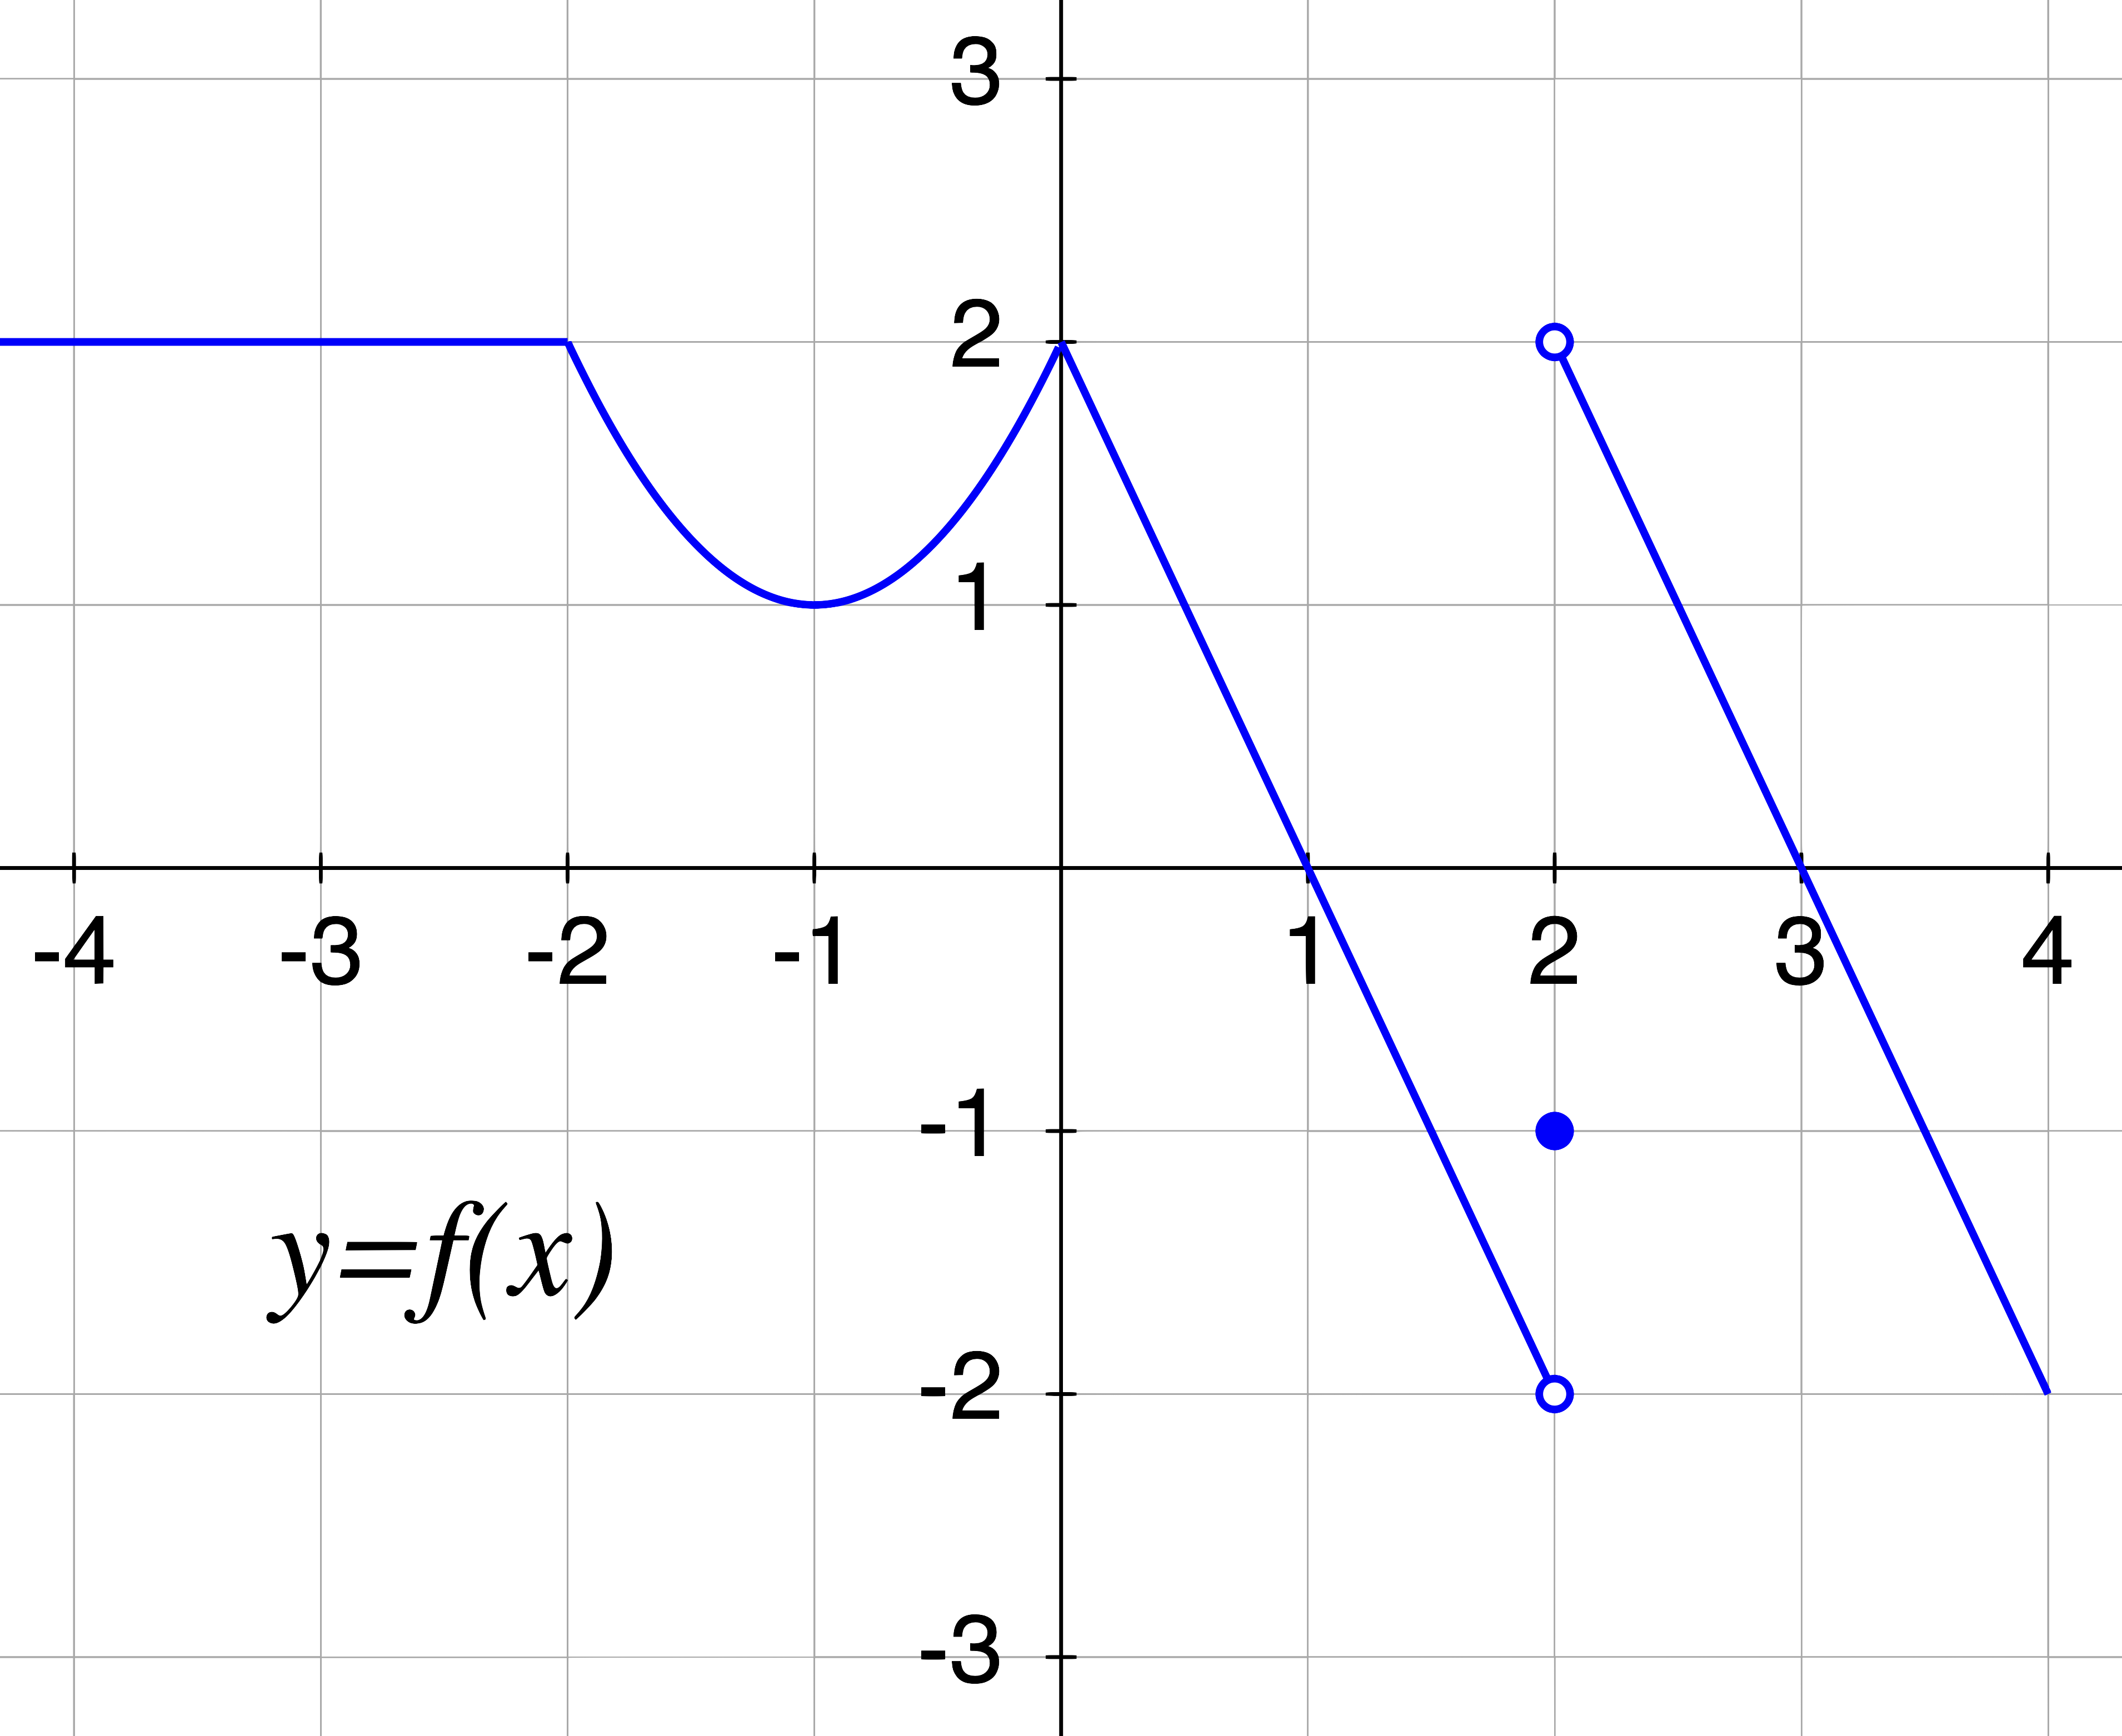
\includegraphics[scale=.4]{EX2a}
				\end{minipage}
				\begin{minipage}{0.2\textwidth}
					Find the value of
					\begin{enumerate}
						\item ${\displaystyle \lim_{x \to 2} f(x)}$

						\item ${\displaystyle \lim_{x \to 0} f(f(x))}$
					\end{enumerate}
				\end{minipage}
			\end{center}
			I ask them to vote (on multiple choice).
		\end{question}
		\begin{comments}
			The vast majority of students confidently answers that none of the limits exists.
			I tell them that I disagree, that the answers to the two questions are different,
			and I invite them to discuss. They are surprised (they were certain to be
			right) and the class immediately erupts in discussion.

			{\parskip=0.5\baselineskip After a while I ask them to vote again. If most of the students got it, I may ask one of them to explain it. But often they are still confused. Then I may use the following hint. I ask why the first limit does not exist. They tell me the side limits are different. So I write the four side limits on the board ${\displaystyle \lim_{x \to 2^+} f(x)}$, ${\displaystyle \lim_{x \to 2^-} f(x)}$, ${\displaystyle \lim_{x \to 0^+} f(f(x))}$, and ${\displaystyle \lim_{x \to 0^-} f(f(x))}$ and ask them to compute them. They discuss with each other again. Without giving them the answer to the side limits, I ask them to vote on ${\displaystyle \lim_{x \to 0} f(f(x))}$ again.

			Perhaps more of the students have the right answer now, but not enough. That tells me they need another bit of help. I ask them to compute ${\displaystyle f(f(0.1))}$, ${\displaystyle f(f(-0.1))}$ and try again. More time to discuss with each other. We vote again. This time I am satisfied with how many got the right answer. Since this question was particularly tough and they worked hard, I will solve the question myself now. They earned it, and by now my explanation will be so much more useful than if I had solved the problem right away, like I would have done in a lecture.

			On the other hand, if students got the first question right immediately, or if I want further practice, I can follow up with a more challenging question. I give them the graph of a function $g$ and ask them to evaluate the limits below. }

			\vspace{.5cm}

			\begin{center}
				\hspace{2cm}
				\begin{minipage}{0.6\textwidth}
					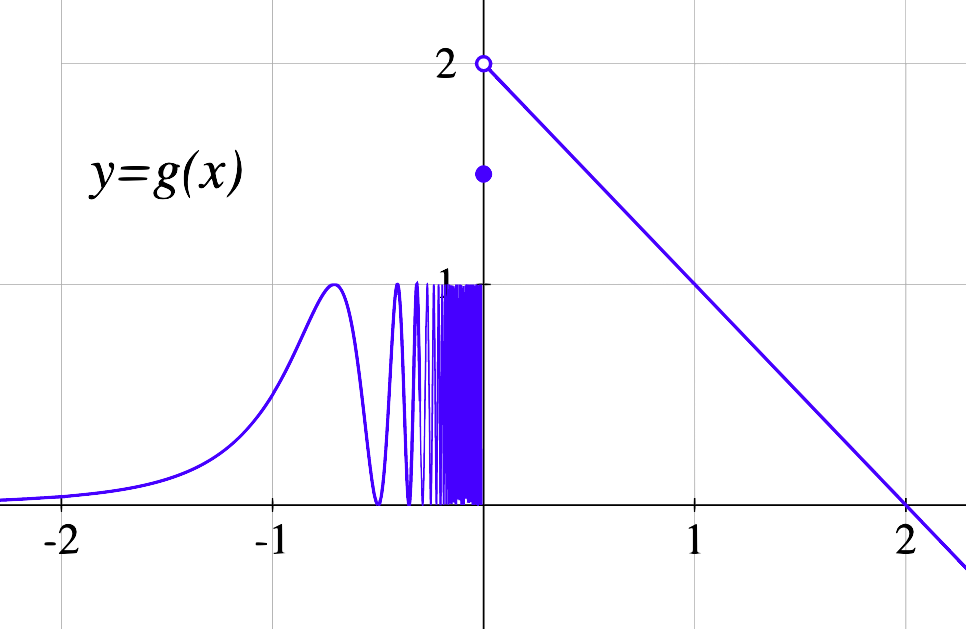
\includegraphics[scale=.3]{EX2b}
				\end{minipage}
				\begin{minipage}{0.2\textwidth}
					Find the value of
					\begin{enumerate}
						\item ${\displaystyle \lim_{x \to 0^+} g(x)}$

						\item ${\displaystyle \lim_{x \to 0^+} \; \lfloor g(x) \rfloor}$

						\item ${\displaystyle \lim_{x \to 0^+} g(\lfloor x \rfloor)}$

						\item ${\displaystyle \lim_{x \to 0^-} g(x)}$

						\item ${\displaystyle \lim_{x \to 0^-} \; \lfloor g(x) \rfloor}$

						\item ${\displaystyle \lim_{x \to 0^-} \; \lfloor \frac{g(x)}{2} \rfloor}$

						\item ${\displaystyle \lim_{x \to 0^-} g(\lfloor x \rfloor)}$
					\end{enumerate}
				\end{minipage}
			\end{center}

			\vspace{.5cm}

			However, if I find the first question was pushing them enough, I will not use
			this second question.

			This is an example of how I react and change my plans based on how they are
			doing.
		\end{comments}
	\end{example}

	%==================
	%==================
	\newpage

	True-False questions, or ``Which ones of these statements are equivalent to..."-questions
	work very well in this format. Students seem to like them.

	\vspace{.5cm}
	\begin{example}
		This is a typical example of finding all the equivalent statements.
		\begin{background}
			Students just learned the definition of limit of a sequence. It is late in
			the course, so by now they can handle formal statements better than earlier.
		\end{background}

		\begin{question}
			Let ${\displaystyle \{a_n\}_{n=0}^{\infty}}$ be a sequence. Let
			${\displaystyle L \in \mathbb{R}}$. \\ Which statements are equivalent to ${\displaystyle ``\{a_n\}_{n=0}^{\infty} \longrightarrow L"}$?

			\begin{enumerate}
				\item ${\displaystyle \forall \varepsilon>0, \; \exists n_0 \in \mathbb{N} \text{ s.t. } \forall n \in \mathbb{N}, \; \quad n \geq n_0 \implies |L-a_n| < \varepsilon.}$

				\item ${\displaystyle \forall \varepsilon>0, \; \exists n_0 \in \mathbb{N} \text{ s.t. } \forall n \in \mathbb{N}, \; \quad n \; {\color{red}  > } \; n_0 \implies |L-a_n| < \varepsilon.}$

				\item ${\displaystyle \forall \varepsilon>0, \; \exists n_0 \in {\color{red} \mathbb{R}} \text{ s.t. } \forall n \in \mathbb{N}, \; \quad n \geq n_0 \implies |L-a_n| < \varepsilon.}$

				\item ${\displaystyle \forall \varepsilon>0, \; \exists n_0 \in \mathbb{N} \text{ s.t. } \forall n \in {\color{red}  \mathbb{R}}, \; \quad n \geq n_0 \implies |L-a_n| < \varepsilon.}$

				\item ${\displaystyle \forall \varepsilon>0, \; \exists n_0 \in \mathbb{N} \text{ s.t. } \forall n \in \mathbb{N}, \; \quad n \geq n_0 \implies |L-a_n| \; {\color{red} \leq} \; \varepsilon.}$

				\item ${\displaystyle \forall \varepsilon \; {\color{red} \in (0,1)}, \; \exists n_0 \in \mathbb{N} \text{ s.t. } \forall n \in \mathbb{N}, \; \quad n \geq n_0 \implies |L-a_n| < \varepsilon.}$

				\item ${\displaystyle \forall \varepsilon>0, \; \exists n_0 \in \mathbb{N} \text{ s.t. } \forall n \in \mathbb{N}, \; \quad n \geq n_0 \implies |L-a_n| < {\color{red} \frac{1}{\varepsilon}}.}$

				\item ${\displaystyle \forall {\color{red} k \in \mathbb{Z}^{+} }, \; \exists n_0 \in \mathbb{N} \text{ s.t. } \forall n \in \mathbb{N}, \; \quad n \geq n_0 \implies |L-a_n| < {\color{red} k}.}$

				\item ${\displaystyle \forall {\color{red} k \in \mathbb{Z}^{+} }, \; \exists n_0 \in \mathbb{N} \text{ s.t. } \forall n \in \mathbb{N}, \; \quad n \geq n_0 \implies |L-a_n| < {\color{red} \frac{1}{k}}.}$
			\end{enumerate}
		\end{question}

		\begin{comments}
			First, I tell them to work individually. I walk among them and I see how they
			are doing. I can see every time they record a ``T" or ``F" on their paper,
			so I see their pace. Once I decide it is time (most have probably not finished
			yet) I ask them to vote. For a few of them there will be consensus. I
			record those answers on the board and will not explain or discuss them. But
			for others there is disagreement or they are reluctant to answer (which
			means they do not know). So I point out the questions we do not have
			consensus on yet and tell them to discuss those with their neighbours. After
			a while we vote on just those again. Based on their replies, I will decide
			what to do. If at some point I think they are slowing down and they need a
			boost of energy, a good hint to restart the discussion is how many correct
			statements there are.
		\end{comments}
	\end{example}

	%==================
	%==================
	\newpage

	\subsection{Explorations}

	Sometimes I use longer questions, perhaps even vague or open-ended, where I
	want students to explore and play with a problem to ``discover" a result, a
	formula, an algorithm, or a concept. These questions are a bit harder to pull off,
	but extremely satisfying when they work, both for students and for us.

	\begin{example}
		This example contains a question about asymptotes with a hidden secondary goal.

		\begin{background}
			Students had watched a video of an example of how to compute the asymptotes
			of a function given its equation.
		\end{background}
		\begin{question}
			In class I gave them this question:
			\begin{center}
				This is the graph of $y = R(x)$. $R$ is a rational function (a quotient of
				polynomials). Find its equation.\\

				\vspace{3mm}
				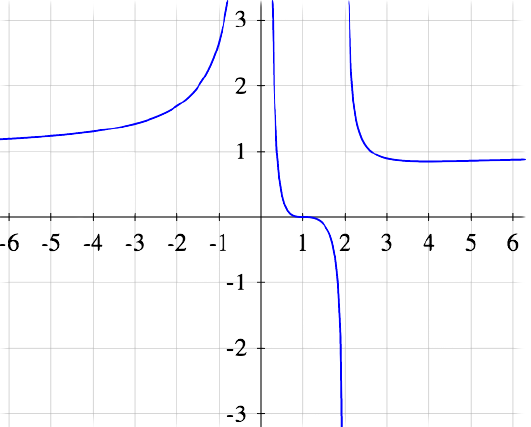
\includegraphics[scale=.45]{EX4}
			\end{center}
			I told them to go to Desmos in their devices and to test their hypotheses.
			They love that!
		\end{question}
		\begin{comments}
			{\parskip=0.3\baselineskip My apparent goal for this question was to discover how the roots in denominator and numerator, and their multiplicity, affect the shape of the graph. But I had a more important goal in mind. I wanted students to practice their problem-solving skills, to be comfortable making and testing conjectures, exploring, being creative, and basically researching. I wanted them to experience the joy of discovering math.

			I was not prepared for how well this worked out.\footnote{Not all questions work this well, but this shows that it is worth it for us to experiment, even if a question may sometimes flop.} There quickly was a lot of energy in the class and students were enthusiastic. Many groups had animated discussions with plenty of ``aha"-moments I even saw some high fives among them when they had a breakthrough. After 10 minutes, I asked if they were ready to discuss the question, or whether they wanted more time. They very firmly asked for more time. This was a good sign, as normally students would prefer me to explain solutions if asked. So I changed my plan, I wrote a challenge question on the board for those who had finished, and let the rest keep working. I could hardly keep up with the many group of students who were calling me to show me their work or ask me questions. }
		\end{comments}
	\end{example}

	%==================
	%==================
	\newpage

	Sometimes an opportunity presents itself serendipitously.

	\begin{example}
		This is an example of a question that I created based on students inquiries.
		\begin{background}
			Students had watched a video where I explained how to use Lagrange's Remainder
			Theorem to bound the error of a Taylor polynomial and, as an application, how
			to prove that ${\displaystyle f(x)=e^x}$ was analytic at $a=0$. In class, I
			guided them through proving that ${\displaystyle f(x)=\sin x}$ was analytic
			at $a=0$. In the process, some students were starting to notice a pattern and
			were inquiring about a general theorem.
		\end{background}
		\vspace{-2mm}
		\begin{question}
			After the exercise, I improvised and wrote the following on the board
			\begin{center}
				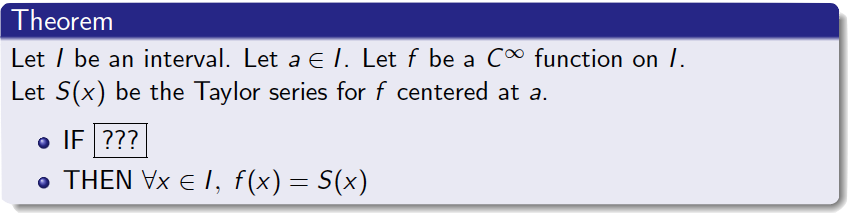
\includegraphics[width=0.65\textwidth]{EX5}
			\end{center}
			\vspace{-3mm}
			I asked them to come up with a condition to replace $???$ that would make
			this theorem true.
		\end{question}
		\vspace{-2mm}
		\begin{comments}
			After discussion among themselves, students were answering ``the
			derivatives have to be bounded". I asked them to formalize this as a very
			precise statement. I had to prod them some more so they would remember to quantify
			all their variables. As I walked among them, I took note of who had interesting
			answers (both right and wrong ones). I asked them to share their answers (sometimes
			calling on them directly) and I copied them on the board. They gave me some
			answers like
			\begin{enumerate}
				\item ${\displaystyle \forall n \in \mathbb{N}, \forall x \in I}$,
					$f^{(n)}$ is bounded between $x$ and $a$.

				\item ${\displaystyle \forall n \in \mathbb{N}, \forall x \in I}$,
					$\exists M \in \mathbb{R}$ such that $\forall \xi$ between $x$ \emph{\&}
					$a$, $| f^{(n)}(\xi)| < M$

				\item ${\displaystyle  \forall x \in I}$, $\exists M \in \mathbb{R}$
					such that $\forall n \in \mathbb{N}$, $\forall \xi$ between $x$ \emph{\&}
					$a$, $| f^{(n)}(\xi)| < M$

				\item ${\displaystyle  \forall x \in I}$, $\exists A, B \in \mathbb{R}$
					such that $\forall n \in \mathbb{N}$, $\forall \xi$ between $x$ \emph{\&}
					$a$, $A < f^{(n)}(\xi) < B$

				\item ${\displaystyle  \forall x \in I}$, $\exists A, B \in \mathbb{R}$
					such that $\forall n \in \mathbb{N}$, $A < f^{(n)}(x) < B$
			\end{enumerate}
			I told them to discuss with their neighbours which one or ones would be valid
			answers. Then they voted. They had already come to a consensus on the correct
			ones, so I asked someone to explain to the class why, and they did.

			Next, I noticed that since various answers were right we had various
			correct theorems, and I asked them to consider ``Which of the correct theorems
			is the most useful one?" In particular, they had to figure out what ``useful"
			meant. I wanted them to realize that the theorem with the weakest
			hypotheses would be the most useful. The discussion continued some more.
			At the end I told them the definition of ``uniformly bounded" (they had
			already discovered the concept, they just needed a name for it).

			Through this exercise, students got a first taste of what research is like:
			coming up with an interesting question, moving from examples to a general case,
			writing precise statements, testing their hypotheses, coming up with new
			theorems.
		\end{comments}
	\end{example}

	%==================
	%==================
	\newpage

	\subsection{Warm-ups}

	I often like to begin with a warm-up question. This is a quick question that requires
	no explanation, that students can jump on working right away, and that should be
	no problem to any student who is trying to do their part. If I begin my class
	at 9:10am, I want the question up and students working on it by 9:11am, and
	the question fully resolved (and we have moved on) by 9:15am. This also establishes
	that the class has officially started, and everybody is immediately active and
	participating.\\

	Sometimes the warm-up question can be a review, and this serves an additional
	purpose. Early in the semester, it is a good idea to use warm-up questions
	that are very similar to the examples in the videos so that you know whether
	students are watching the videos or not. If many students don't answer or answer
	incorrectly, this will be a great opportunity to remind them of the importance
	of watching the videos before class.

	\begin{example}
		This is simple question designed to help students determine whether they understand
		some basic concepts or not.
		\begin{background}
			In the previous classes we had learned about improper integrals, the main
			family of examples, of the Limit-Comparison Test. Today we are working on
			something new, but first we begin with this review question
		\end{background}
		\begin{question}
			I asked students whether the following integrals are convergent and divergent.
			%
			\begin{center}
				\begin{minipage}{0.7\textwidth}
					\begin{multicols}{2}
						\begin{enumerate}
							\item ${\displaystyle \int_1^\infty \frac{1}{x^{2}} \, dx}$

							\item ${\displaystyle \int_1^\infty \frac{1}{x} \, dx}$

							\item ${\displaystyle \int_1^\infty \frac{1}{\sqrt{x}} \, dx}$

							\item ${\displaystyle \int_1^\infty \frac{x+1}{x^{3}+2} \, dx}$

							\item ${\displaystyle \int_1^\infty \frac{\sqrt{x^{2}+5}}{x^{2}+6} \, dx}$

							\item ${\displaystyle \int_1^\infty \frac{x^{2}+3}{\sqrt{x^{5}+2}} \, dx}$
						\end{enumerate}
					\end{multicols}
				\end{minipage}
			\end{center}
			\vspace{1mm}
		\end{question}

		\begin{comments}
			{\parskip=0.5\baselineskip I give students two minutes to think, and then I ask them to vote. By this time of the course\footnote{It takes quite some training and prodding, to get to this point.} I have them trained so I can say ``Everybody answer loudly together. Is it convergent, yes or no? Number 1?" (they answer) ``Number 2?" (they answer) ... I am hoping that the majority has gotten the right answer and then I move on without further discussion.

			What is the point of this question? We had worked on much more complicated examples earlier, but these are the basic ones, the ones we want all students to know confidently and quickly, the ones they are going to build up on later. They should not be moving to the next unit without this. In general, it is easy for a student to fall behind and convince themselves that ``It is okay. Everybody is equally confused." By resolving this question with all students answering loudly, I am making it apparent to those who are behind that no, that is not happening to everyone, and any student who is doing their part is getting at least this question. In later questions everybody will be equally confused, but for this one they should not be.

			Of course, if I miscalculated, I can always convert this question into a regular Think-Pair-Share.}
		\end{comments}
	\end{example}

	%==================
	%==================
	\newpage

	\subsection{Computations}
	{\parskip=0.5\baselineskip While we normally prefer to use class time for conceptual questions, there is room for a bit of computational practice every now and then. We do want students to gain some fluency after all.

	When we do computational practice, I normally post a bunch of questions at once and give them a good chunk of time, while I walk around them, check on what they are doing, and answer their questions. Depending on how they are doing I decide how much time I have to wait, whether they are on top of things and I can move on, or I should solve an example myself, or point out a common error, or something else. I never feel the need to go through all the problems. Normally the last question is a harder one to slow down the fastest students, and I do not care if most students do not get to it (I do remind them of this). I will only discuss problems that most of them have worked on.

	I suggest you avoid the temptation of spending a lot of time working through many examples in detail yourself. That is what the videos are for. Moreover, students have access to literally thousands of other worked-out examples with a simple search on YouTube. Remember that is is not necessary for you to ``cover" all the heuristics, even though you will likely feel the need to.\\ }

	\begin{example}
		This example has computational questions with different levels of difficulty
		including one hard question to keep busy the students that found everything else
		too easy.
		%
		\begin{background}
			Students had learned the Ratio Test for convergence of series in a video and
			watched a couple of examples.
		\end{background}
		\begin{question}
			In class, I asked students to use the Ratio Test to decide which of the
			following series are convergent:
			\begin{center}
				\begin{minipage}{0.7\textwidth}
					\begin{multicols}{2}
						\begin{enumerate}[label=(\arabic{*})]
							\item ${\displaystyle \sum_{n=1}^\infty \frac{3^{n}}{n!}}$ \label{sum1}

							\item ${\displaystyle \sum_{n=1}^\infty \frac{(2n)!}{n!^{2} 3^{n+1}}}$
								\label{sum2}

							\item ${\displaystyle \sum_{n=2}^\infty \frac{1}{\ln n}}$ \label{sum3}

							\item ${\displaystyle \sum_{n=2}^\infty \frac{n!}{n^{n}}}$ \label{sum4}
						\end{enumerate}
					\end{multicols}
				\end{minipage}
			\end{center}

			\vspace{1mm}
		\end{question}
		\begin{comments}
			I began by giving them 10 full minutes to work on while I walked among them
			and talked to some of them. They were proceeding slower than I thought\footnote{We
			always forget what is like doing things for the first time}. Most students
			(the ones who had watched the videos at least) could solve \ref{sum1}, perhaps
			slowly, perhaps discussing with friends, and perhaps rereading their notes
			or rewatching the video in their tablets. There were some errors in
			\ref{sum2}, some did not know what to do in \ref{sum3} after the test is found
			inconclusive, and few of them had gotten to \ref{sum4}.

			{\parskip=0.5\baselineskip I told them that I saw consensus that \ref{sum1} was convergent and we were going to move on. I told them I would discuss instead only \ref{sum2} and \ref{sum3}, to take a bit more time, and to discuss with their neighbours if they had not done so. After a while, I explained the common error I had seen in their answers to \ref{sum2}, and I led a discussion of what to do with \ref{sum3}. I did not touch \ref{sum4}; it was there to keep busy the students that found everything else too easy. }
		\end{comments}
	\end{example}

	%==================
	%==================
	\newpage

	\subsection{Proofs}

	Learning to read, understand, critique, and write proofs is one of the major learning
	objectives of the course, so it makes sense to spend some class time on it. Alas,
	this is the most difficult skill to tackle. I will explain the tools I normally
	use, although I acknowledge this is what I am least confident on.

	{\parskip=0.5\baselineskip First, what not to do. It is tempting to spend large amounts of time writing full proofs on the board in detail while students copy them. But that is a lecture, not active learning. Students already have that in the videos (which they can rewind, pause, and rewatch). If they want more examples of detailed proofs, they can find tons online or in the textbook. Instead, we want them to start writing proofs themselves. They will struggle, because they find this difficult, and they will be insecure, because they do not know if they are right. But if you manage to make them spend time actively trying, you have already succeeded.

	The simplest activity I use is to give students a simple claim, some guidance on the proof, and ask them to write it out in full.\\ }

	\begin{example}
		In this example, I give students the steps that they need to follow to
		complete a proof. I hope they can follow them and gain some confidence.
		\begin{background}
			Students have watched a few proofs with the same concepts in the videos.
		\end{background}
		\begin{question}
			We want to prove this theorem
			\begin{center}
				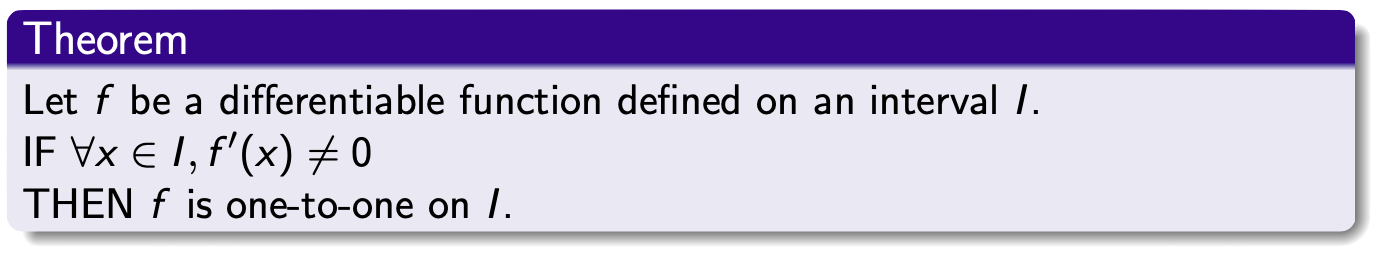
\includegraphics[width=0.7\textwidth]{EX8}

				\vspace{.5cm}

				\begin{minipage}{0.7\textwidth}
					Follow these steps to write down the proof:
					\begin{enumerate}
						\item Transform \quad ${\displaystyle [P \implies Q]}$ \quad into \quad
							${\displaystyle  [(\text{not } Q) \implies (\text{not } P)]}$. \\
							You get an equivalent Theorem (call it ``Theorem 2"). \\ We are
							going to prove Theorem 2 instead.

						\item Write the definition of ``$f$ is not one-to-one on $I$". You will
							need it.

						\item Recall the statement of Rolle's Theorem. You will need it.

						\item Do some rough work if needed.

						\item Write a complete proof for Theorem 2.
					\end{enumerate}
				\end{minipage}
			\end{center}
			
\includegraphics[height=12pt]{alert.png}
			\textbf{\textcolor{137cp3}{Warning:}} students will be much slower than
			you expect.
		\end{question}
		\begin{comments}
			Even if I simply give them this activity, wait for them to write the proof,
			and after that I write the proof myself on the board, this is going to be
			much more useful than writing multiple proofs by myself on the board
			without them having participated.
		\end{comments}
	\end{example}

	%==================
	%==================

	\newpage

	{Taking it a step further, sometimes I first ask them to write a proof (with guidance), and then I help them to check the proof for correctness, and give each other's feedback. }

	\begin{example}
		The goal of this activity is for student to give each other feedback on their
		proof writing.
		\begin{background}
			Students have watched a video that explains how to come up with, and write
			a full proof of the limit law for sums.
		\end{background}
		\begin{question}
			First I give them this activity in class
			\begin{center}
				\begin{minipage}{0.8\textwidth}
					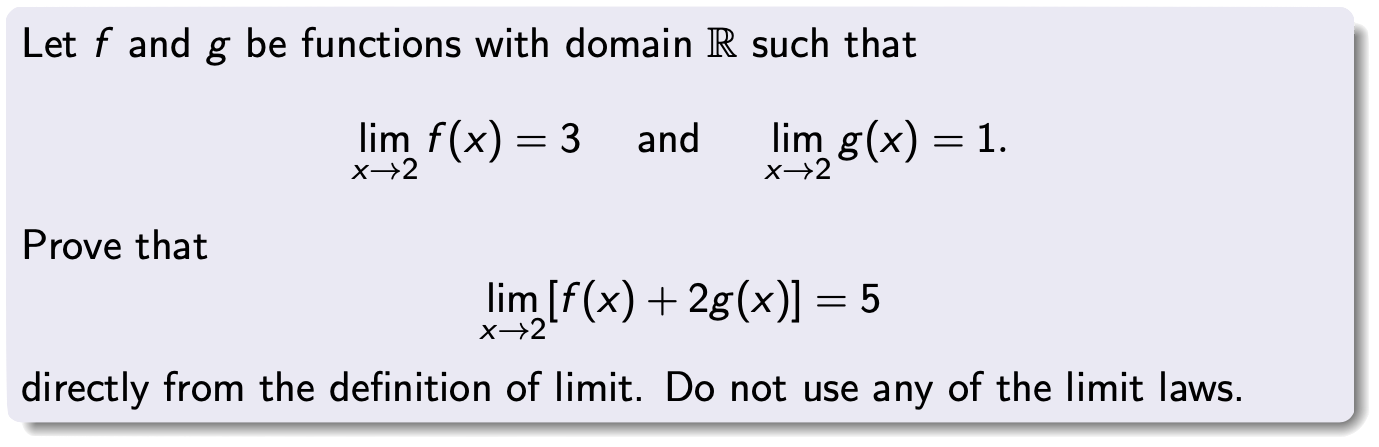
\includegraphics[width=0.85\textwidth]{EX9}
					\begin{enumerate}
						\item Write down the formal definition of the statement you want to prove.

						\item Write down what the structure of the formal proof should be,
							without filling the details.

						\item Rough work.

						\item Write down a complete proof.
					\end{enumerate}
				\end{minipage}
			\end{center}
		\end{question}
		\begin{comments}
			Notice that it is very similar to what they saw in the video. There is no
			value in me writing a proof for this at all. (They can rewatch the video!)
			Rather, today we are going to practice how to criticize proofs and give feedback.
			Once I have given them enough time and many have a draft, I ask them to pair
			up, trade proofs, and give each other feedback following these prompts:
			\begin{center}
				\begin{minipage}{0.8\textwidth}
					\begin{enumerate}
						\item Is the structure of the proof correct? (First fix $\varepsilon$,
							then choose $\delta$, then ...)

						\item Did you say exactly what $\delta$ is?

						\item Is the proof self-contained? (I do not need to read the rough work)

						\item Are all variables defined? In the right order?

						\item Do all steps follow logically from what comes before? Do you
							start from what you know and prove what you have to prove?

						\item Are you assuming the conclusion?
					\end{enumerate}
				\end{minipage}
			\end{center}I hope they get comfortable with writing proofs together and checking
			each other's proofs. It will be valuable when they study.
		\end{comments}
	\end{example}

	%==================
	%==================

	\newpage

	An activity that students seem to enjoy a lot is ``Find the error in this
	proof".

	\begin{example}
		Learning to identify a common error.
		\begin{background}
			This is part of learning to prove that a limit exists from the definition.
		\end{background}
		\begin{question}
			I give student this question
			\begin{center}
				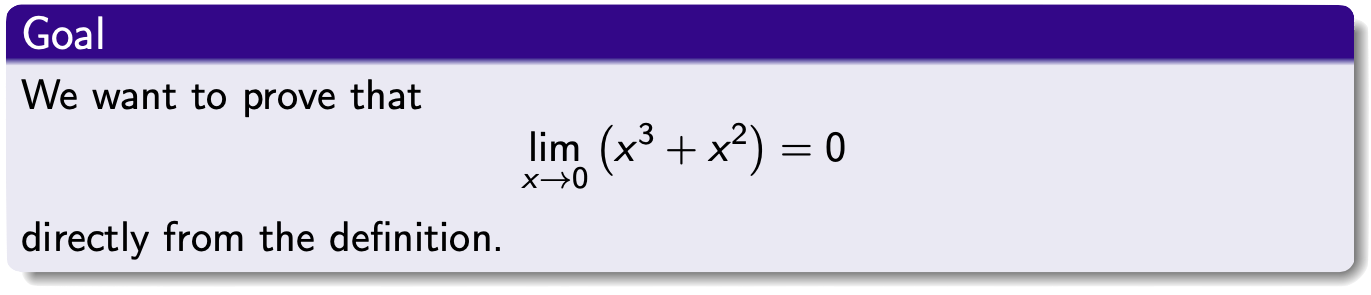
\includegraphics[width=0.8\textwidth]{EX10a}
			\end{center}
			together with some guidance on the proof (which I am omitting now). Then I
			ask them to discuss with each other. After that, I ask them to find the
			error in this proof
			\begin{center}
				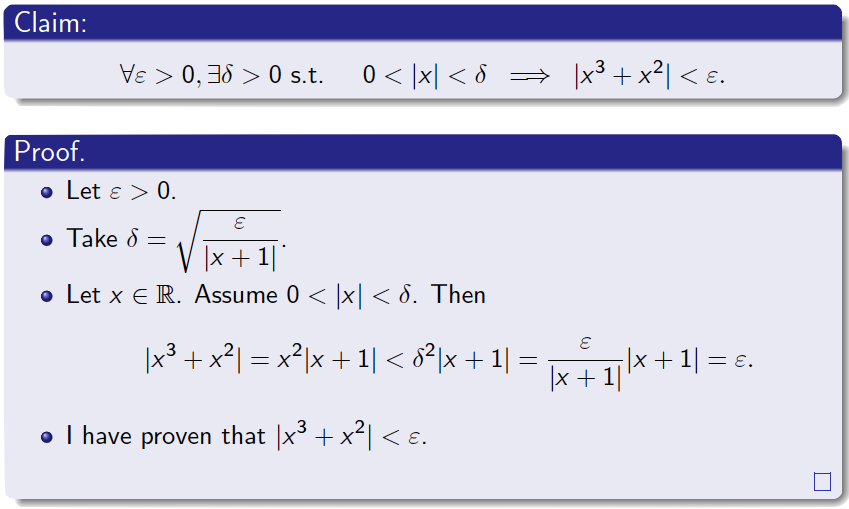
\includegraphics[width=0.8\textwidth]{EX10b}
			\end{center}
		\end{question}
		\begin{comments}
			This is an error students make very often, and I am certain many of them
			have made it today. I invite them to discuss the question with each other.
			Once I am satisfied that enough of them have realized the error, I ask them
			to explain it to the class. I hope this makes it more memorable, they learn
			not to do this in the future, and they learn to find this error when they
			are checking each other's proofs. I do not write the details of this proof
			in the board.
		\end{comments}
	\end{example}

	%==================
	%==================
\end{document}
